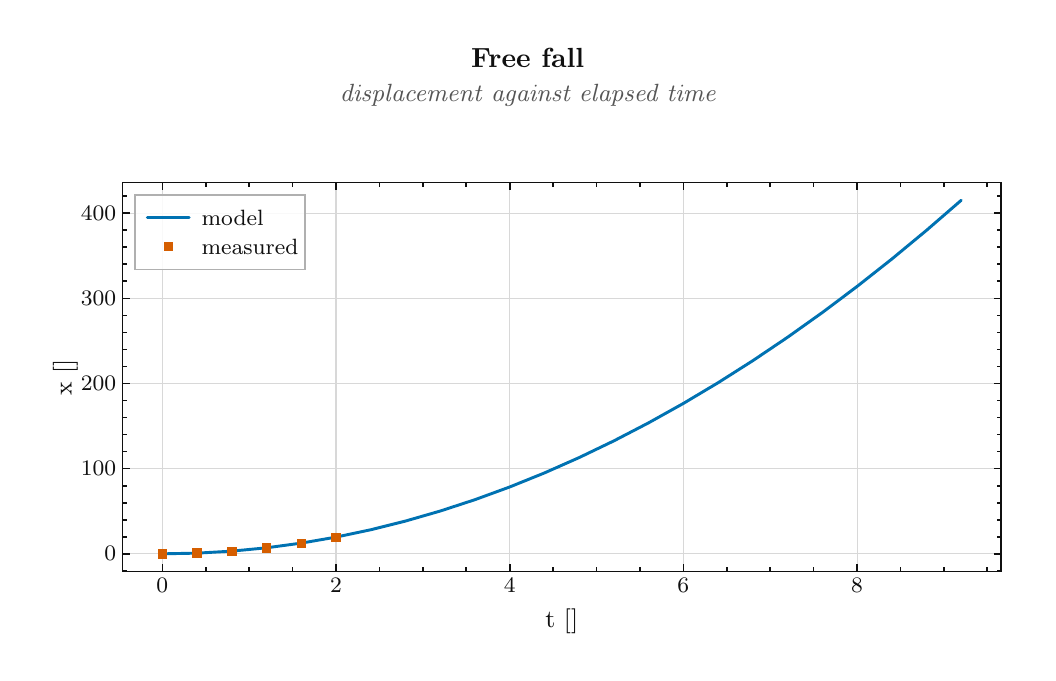
\begin{tikzpicture}[every node/.style={inner sep=0bp,outer sep=0bp}]
  \definecolor{qcA}{rgb}{1,1,1}
  \definecolor{qcB}{rgb}{0.062745,0.062745,0.062745}
  \definecolor{qcC}{rgb}{0.333333,0.333333,0.333333}
  \definecolor{qcD}{rgb}{0.847059,0.847059,0.847059}
  \definecolor{qcE}{rgb}{0,0.447059,0.698039}
  \def\mareymarkF#1#2{\path[fill,shift={(#1,#2)}] (-1.688bp,-1.688bp) rectangle (1.688bp,1.688bp);}
  \definecolor{qcG}{rgb}{0.835294,0.368627,0}
  \definecolor{qcH}{rgb}{0.690196,0.690196,0.690196}
  \useasboundingbox (0bp,0bp) rectangle (360bp,225bp);
  % marey-key: figure
  \path[fill=qcA] (0bp,0bp) -- (360bp,0bp) -- (360bp,225bp) -- (0bp,225bp) -- cycle;
  % marey-role: annotation -- Free fall
  \node[anchor=north,text=qcB,font=\bfseries\fontsize{10}{12}\selectfont] at (180bp,217.5bp) {Free fall};
  \node[anchor=north,text=qcC,font=\itshape\fontsize{9}{10.8}\selectfont] at (180bp,204.5bp) {displacement against elapsed time};
  % marey-key: figure/panel-0-0
  % marey-role: other:panel -- panel
  % marey-data: row = 0
  % marey-data: col = 0
  % marey-data: layers = 2
  % marey-data: x-tick-rule = all
  % marey-data: y-tick-rule = all
  % marey-key: figure/panel-0-0/grid
  % marey-role: decoration -- gridlines
  % marey-data: lines = 10
  \path[draw=qcD,line width=0.375bp] (48.481bp,29.225bp) -- (48.481bp,169.225bp) (111.001bp,29.225bp) -- (111.001bp,169.225bp) (173.522bp,29.225bp) -- (173.522bp,169.225bp) (236.042bp,29.225bp) -- (236.042bp,169.225bp) (298.562bp,29.225bp) -- (298.562bp,169.225bp) (34.101bp,35.589bp) -- (350.454bp,35.589bp) (34.101bp,66.245bp) -- (350.454bp,66.245bp) (34.101bp,96.901bp) -- (350.454bp,96.901bp) (34.101bp,127.558bp) -- (350.454bp,127.558bp) (34.101bp,158.214bp) -- (350.454bp,158.214bp);
  \begin{scope}
    \clip (34.101bp,29.225bp) -- (350.454bp,29.225bp) -- (350.454bp,169.225bp) -- (34.101bp,169.225bp) -- cycle;
    % marey-key: figure/panel-0-0/layer-0
    % marey-role: series -- model
    % marey-data: series = model
    % marey-data: points = 24
    \path[draw=qcE,line width=1.05bp,line cap=round,line join=round] (48.481bp,35.589bp) -- (60.985bp,35.829bp) -- (73.489bp,36.551bp) -- (85.993bp,37.754bp) -- (98.497bp,39.438bp) -- (111.001bp,41.603bp) -- (123.505bp,44.25bp) -- (136.009bp,47.378bp) -- (148.514bp,50.986bp) -- (161.018bp,55.077bp) -- (173.522bp,59.648bp) -- (186.026bp,64.7bp) -- (198.53bp,70.234bp) -- (211.034bp,76.249bp) -- (223.538bp,82.745bp) -- (236.042bp,89.722bp) -- (248.546bp,97.18bp) -- (261.05bp,105.119bp) -- (273.554bp,113.54bp) -- (286.058bp,122.442bp) -- (298.562bp,131.825bp) -- (311.066bp,141.689bp) -- (323.57bp,152.035bp) -- (336.074bp,162.861bp);
    % marey-key: figure/panel-0-0/layer-1
    % marey-role: series -- measured
    % marey-data: series = measured
    % marey-data: points = 6
    \begin{scope}[fill=qcG]
      \mareymarkF{48.481bp}{35.589bp}
      \mareymarkF{60.985bp}{35.824bp}
      \mareymarkF{73.489bp}{36.53bp}
      \mareymarkF{85.993bp}{37.708bp}
      \mareymarkF{98.497bp}{39.356bp}
      \mareymarkF{111.001bp}{41.475bp}
    \end{scope}
  \end{scope}
  % marey-key: figure/panel-0-0/axis-x
  % marey-role: axis -- t [s]
  % marey-data: side = bottom
  % marey-data: unit = s
  % marey-data: prefix =
  % marey-data: ticks = 5
  % marey-data: tick-rule = all
  \path[draw=qcB,line width=0.6bp] (48.481bp,31.85bp) -- (48.481bp,29.225bp) (111.001bp,31.85bp) -- (111.001bp,29.225bp) (173.522bp,31.85bp) -- (173.522bp,29.225bp) (236.042bp,31.85bp) -- (236.042bp,29.225bp) (298.562bp,31.85bp) -- (298.562bp,29.225bp) (64.111bp,30.725bp) -- (64.111bp,29.225bp) (79.741bp,30.725bp) -- (79.741bp,29.225bp) (95.371bp,30.725bp) -- (95.371bp,29.225bp) (126.631bp,30.725bp) -- (126.631bp,29.225bp) (142.262bp,30.725bp) -- (142.262bp,29.225bp) (157.892bp,30.725bp) -- (157.892bp,29.225bp) (189.152bp,30.725bp) -- (189.152bp,29.225bp) (204.782bp,30.725bp) -- (204.782bp,29.225bp) (220.412bp,30.725bp) -- (220.412bp,29.225bp) (251.672bp,30.725bp) -- (251.672bp,29.225bp) (267.302bp,30.725bp) -- (267.302bp,29.225bp) (282.932bp,30.725bp) -- (282.932bp,29.225bp) (314.192bp,30.725bp) -- (314.192bp,29.225bp) (329.822bp,30.725bp) -- (329.822bp,29.225bp) (345.452bp,30.725bp) -- (345.452bp,29.225bp) (48.481bp,166.6bp) -- (48.481bp,169.225bp) (111.001bp,166.6bp) -- (111.001bp,169.225bp) (173.522bp,166.6bp) -- (173.522bp,169.225bp) (236.042bp,166.6bp) -- (236.042bp,169.225bp) (298.562bp,166.6bp) -- (298.562bp,169.225bp) (64.111bp,167.725bp) -- (64.111bp,169.225bp) (79.741bp,167.725bp) -- (79.741bp,169.225bp) (95.371bp,167.725bp) -- (95.371bp,169.225bp) (126.631bp,167.725bp) -- (126.631bp,169.225bp) (142.262bp,167.725bp) -- (142.262bp,169.225bp) (157.892bp,167.725bp) -- (157.892bp,169.225bp) (189.152bp,167.725bp) -- (189.152bp,169.225bp) (204.782bp,167.725bp) -- (204.782bp,169.225bp) (220.412bp,167.725bp) -- (220.412bp,169.225bp) (251.672bp,167.725bp) -- (251.672bp,169.225bp) (267.302bp,167.725bp) -- (267.302bp,169.225bp) (282.932bp,167.725bp) -- (282.932bp,169.225bp) (314.192bp,167.725bp) -- (314.192bp,169.225bp) (329.822bp,167.725bp) -- (329.822bp,169.225bp) (345.452bp,167.725bp) -- (345.452bp,169.225bp);
  \node[anchor=north,text=qcB,font=\fontsize{8}{9.6}\selectfont] at (48.481bp,26.975bp) {0};
  \node[anchor=north,text=qcB,font=\fontsize{8}{9.6}\selectfont] at (111.001bp,26.975bp) {2};
  \node[anchor=north,text=qcB,font=\fontsize{8}{9.6}\selectfont] at (173.522bp,26.975bp) {4};
  \node[anchor=north,text=qcB,font=\fontsize{8}{9.6}\selectfont] at (236.042bp,26.975bp) {6};
  \node[anchor=north,text=qcB,font=\fontsize{8}{9.6}\selectfont] at (298.562bp,26.975bp) {8};
  \node[anchor=north,text=qcB,font=\fontsize{9}{10.8}\selectfont] at (192.278bp,15.825bp) {t [\qty{}{\second}]};
  % marey-key: figure/panel-0-0/axis-y
  % marey-role: axis -- x [m]
  % marey-data: side = left
  % marey-data: unit = m
  % marey-data: prefix =
  % marey-data: ticks = 5
  % marey-data: tick-rule = all
  \path[draw=qcB,line width=0.6bp] (36.726bp,35.589bp) -- (34.101bp,35.589bp) (36.726bp,66.245bp) -- (34.101bp,66.245bp) (36.726bp,96.901bp) -- (34.101bp,96.901bp) (36.726bp,127.558bp) -- (34.101bp,127.558bp) (36.726bp,158.214bp) -- (34.101bp,158.214bp) (35.601bp,29.457bp) -- (34.101bp,29.457bp) (35.601bp,41.72bp) -- (34.101bp,41.72bp) (35.601bp,47.851bp) -- (34.101bp,47.851bp) (35.601bp,53.982bp) -- (34.101bp,53.982bp) (35.601bp,60.114bp) -- (34.101bp,60.114bp) (35.601bp,72.376bp) -- (34.101bp,72.376bp) (35.601bp,78.508bp) -- (34.101bp,78.508bp) (35.601bp,84.639bp) -- (34.101bp,84.639bp) (35.601bp,90.77bp) -- (34.101bp,90.77bp) (35.601bp,103.033bp) -- (34.101bp,103.033bp) (35.601bp,109.164bp) -- (34.101bp,109.164bp) (35.601bp,115.295bp) -- (34.101bp,115.295bp) (35.601bp,121.426bp) -- (34.101bp,121.426bp) (35.601bp,133.689bp) -- (34.101bp,133.689bp) (35.601bp,139.82bp) -- (34.101bp,139.82bp) (35.601bp,145.952bp) -- (34.101bp,145.952bp) (35.601bp,152.083bp) -- (34.101bp,152.083bp) (35.601bp,164.345bp) -- (34.101bp,164.345bp) (347.829bp,35.589bp) -- (350.454bp,35.589bp) (347.829bp,66.245bp) -- (350.454bp,66.245bp) (347.829bp,96.901bp) -- (350.454bp,96.901bp) (347.829bp,127.558bp) -- (350.454bp,127.558bp) (347.829bp,158.214bp) -- (350.454bp,158.214bp) (348.954bp,29.457bp) -- (350.454bp,29.457bp) (348.954bp,41.72bp) -- (350.454bp,41.72bp) (348.954bp,47.851bp) -- (350.454bp,47.851bp) (348.954bp,53.982bp) -- (350.454bp,53.982bp) (348.954bp,60.114bp) -- (350.454bp,60.114bp) (348.954bp,72.376bp) -- (350.454bp,72.376bp) (348.954bp,78.508bp) -- (350.454bp,78.508bp) (348.954bp,84.639bp) -- (350.454bp,84.639bp) (348.954bp,90.77bp) -- (350.454bp,90.77bp) (348.954bp,103.033bp) -- (350.454bp,103.033bp) (348.954bp,109.164bp) -- (350.454bp,109.164bp) (348.954bp,115.295bp) -- (350.454bp,115.295bp) (348.954bp,121.426bp) -- (350.454bp,121.426bp) (348.954bp,133.689bp) -- (350.454bp,133.689bp) (348.954bp,139.82bp) -- (350.454bp,139.82bp) (348.954bp,145.952bp) -- (350.454bp,145.952bp) (348.954bp,152.083bp) -- (350.454bp,152.083bp) (348.954bp,164.345bp) -- (350.454bp,164.345bp);
  \node[anchor=east,text=qcB,font=\fontsize{8}{9.6}\selectfont] at (31.851bp,35.589bp) {0};
  \node[anchor=east,text=qcB,font=\fontsize{8}{9.6}\selectfont] at (31.851bp,66.245bp) {100};
  \node[anchor=east,text=qcB,font=\fontsize{8}{9.6}\selectfont] at (31.851bp,96.901bp) {200};
  \node[anchor=east,text=qcB,font=\fontsize{8}{9.6}\selectfont] at (31.851bp,127.558bp) {300};
  \node[anchor=east,text=qcB,font=\fontsize{8}{9.6}\selectfont] at (31.851bp,158.214bp) {400};
  \node[anchor=base,text=qcB,rotate=90,font=\fontsize{9}{10.8}\selectfont] at (15.825bp,99.225bp) {x [\qty{}{\metre}]};
  % marey-role: decoration -- panel frame
  \path[draw=qcB,line width=0.6bp] (34.101bp,29.225bp) -- (350.454bp,29.225bp) -- (350.454bp,169.225bp) -- (34.101bp,169.225bp) -- cycle;
  % marey-key: figure/panel-0-0/legend
  % marey-role: legend -- legend
  % marey-data: entries = 2
  \path[fill=qcA,fill opacity=0.85,draw=qcH,line width=0.45bp] (38.601bp,137.925bp) -- (99.824bp,137.925bp) -- (99.824bp,164.725bp) -- (38.601bp,164.725bp) -- cycle;
  % marey-role: other:legend-entry -- model
  % marey-data: series = model
  % marey-data: color = #0072b2
  \path[draw=qcE,line width=1.05bp,line cap=round] (43.101bp,156.525bp) -- (58.101bp,156.525bp);
  \node[anchor=west,text=qcB,font=\fontsize{8}{9.6}\selectfont] at (62.601bp,156.525bp) {model};
  % marey-role: other:legend-entry -- measured
  % marey-data: series = measured
  % marey-data: color = #d55e00
  \begin{scope}[fill=qcG]
    \mareymarkF{50.601bp}{146.125bp}
  \end{scope}
  \node[anchor=west,text=qcB,font=\fontsize{8}{9.6}\selectfont] at (62.601bp,146.125bp) {measured};
\end{tikzpicture}
